\subsection{SWE in Spherical Coordinates}
Until now we have derived the shallow water equations in cartesian coordinates.
In this section, we will derive the shallow water equations in spherical coordinates.
We will follow the methods used in.
To illustrate the spherical coordinates, we will use the latitude and longitude system, visualized in~\autoref{fig:lat-long-earth}.

\begin{figure}[H]
    \centering
    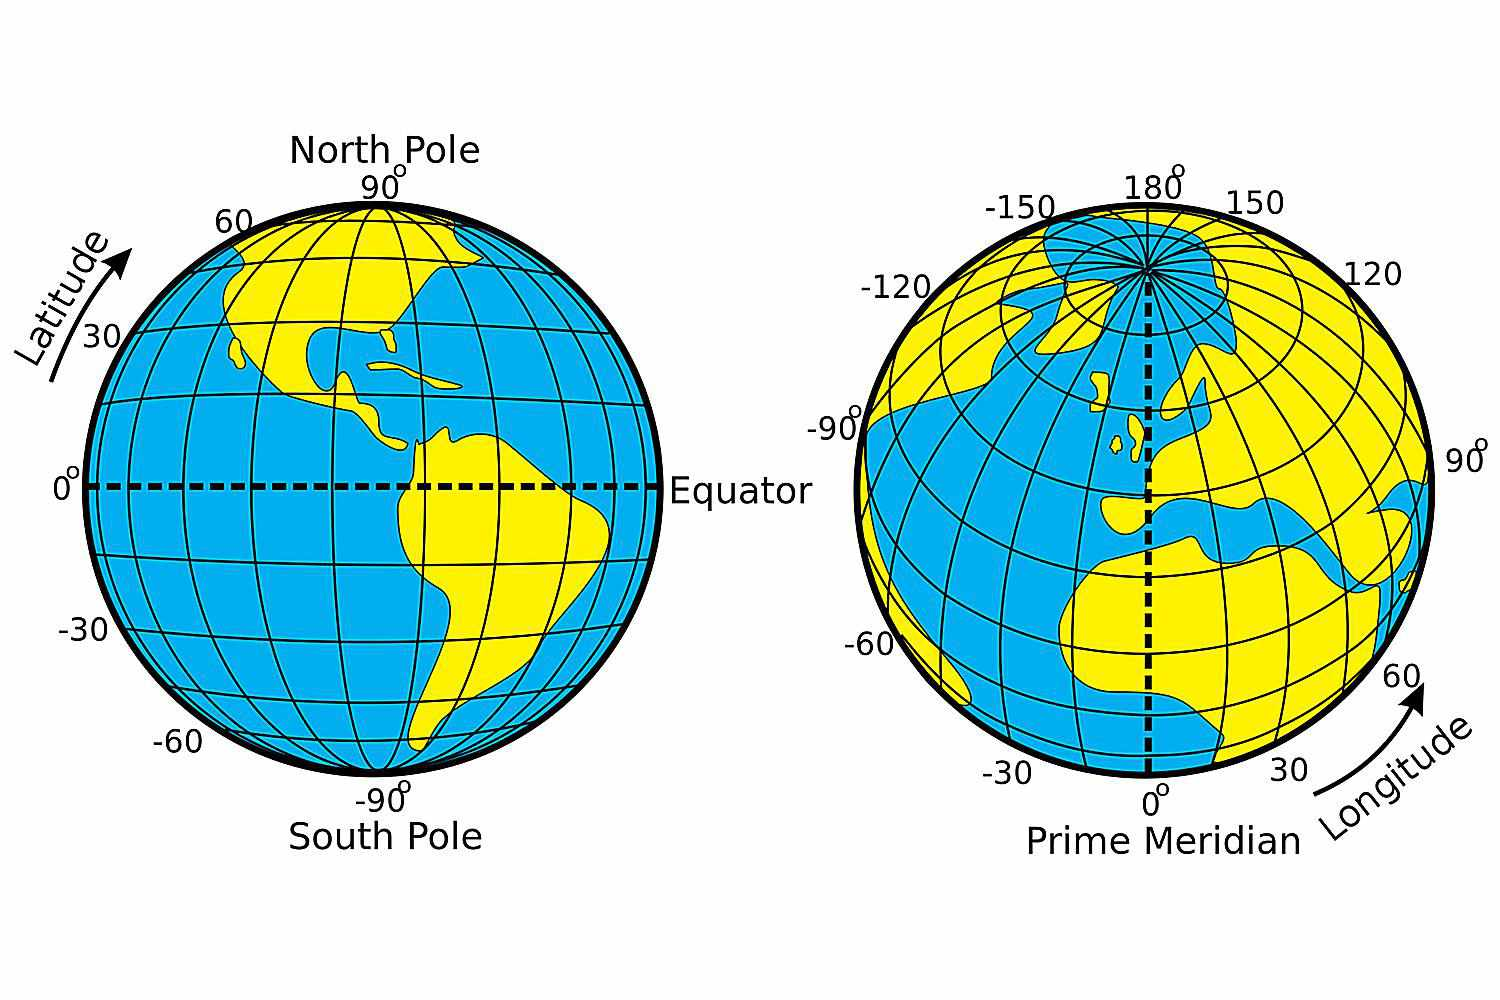
\includegraphics[width=0.5\textwidth]{C:/Users/Matteo/Shallow-Water-Equations/figs/lat-long-earth.jpg}
    \caption{Illustration of latitude and longitude on the planet earth.
    Illustration from~\cite{lat-long-earth}.}\label{fig:lat-long-earth}
\end{figure}
The spherical coordinates we use are ($r$, $\theta$, $\phi$), where $r$ is the radius from the center of the sphere, $\theta$ is the longitude, and $\phi$ is the latitude.
We also refer to $\theta$ as the elevation angle and $\phi$ as the azimuth angle, where $\phi$ goes from $-\frac{\pi}{2}$ at the south pole to $\frac{\pi}{2}$ at the north pole, calculated in radians.
The angle $\theta$ goes from $0$ at the priime meridian, increasing to the east, to $2\pi$ also calculated in radians.
In spherical coordinates any point on the surface of the sphere can be represented by the coordinates ($r$, $\theta$, $\phi$).
We see that the longitude direction ($\theta$) is the east-west component, whereas the latitude direction ($\phi$) is the north-south component.
We consider a small domain of the sphere, as illustrated in \autoref{fig:sphere-small-domain}.
\begin{figure}[H]
    \centering
    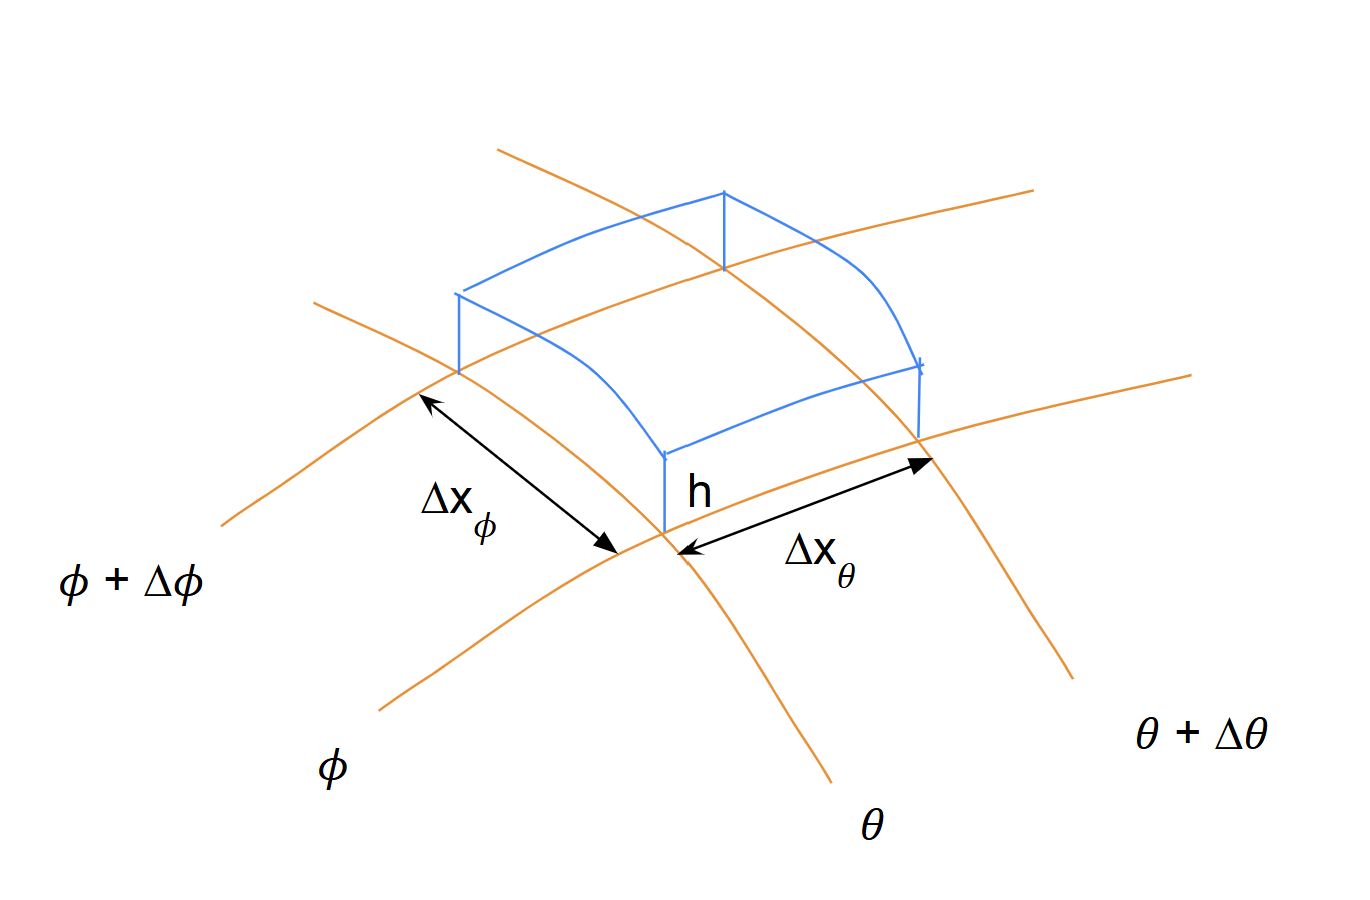
\includegraphics[width=0.5\textwidth]{C:/Users/Matteo/Shallow-Water-Equations/figs/Sphere-small-domain.png}
    \caption{Illustrations of a small domain of the surface of the sphere.}\label{fig:sphere-small-domain}
\end{figure}
We want to find expressions for $\Delta x_{\phi}$ and $\Delta x_{\theta}$, the distances in the $\phi$ and $\theta$ directions, respectively, as illustrated in \autoref{fig:sphere-small-domain}.
We can find these distances by using the arc length formula.
Recall that the circumreference of a full circle is $2\pi r$, where $r$ is the radius of the circle.
The arc length is a fraction of the full circumreference, and it is given by the formula $l = r v$, where $l$ is the arc length, $r$ is the radius, and $v$ is the angle in radians.
Assuming that the planet earth on the latitude side is a circle, we can find the distance $\Delta x_{\phi}$ by using the arc length formula, as:
\begin{align*}
    \Delta x_{\phi} = r \Delta \phi,
\end{align*}
where $\Delta \phi$ is the change in the latitude angle and $r$ is the radius of the sphere.
We assume that the planet earth is a perfect sphere, meaning that the radius is constant.
Considering the longitude dimension $\Delta x_{\theta}$, we need to make some adjustments, as we can see that the circumreference at equator is larger than at the poles.
Meaning that if we conisder the horizontal circle at some given latitude $\phi$, the radius of the circle is $r \cos(\phi)$ (why?).
Using that, together with the formula for the arc length, we can find the distance $\Delta x_{\theta}$ as:
\begin{align*}
    \Delta x_{\theta} = r \cos(\phi) \Delta \theta.
\end{align*}
The volume of a small domain of the sphere is given by 
\begin{align*}
    V &= \Delta x_{\phi} \Delta x_{\theta} h \\
    &= r^2 h \cos(\phi) \Delta \phi \Delta \theta,
\end{align*}
assuming that the height of the domain is $h$, and that the domain is rectangular.
This is a fair assumption for small values of $\Delta x_{\phi}$ and $\Delta x_{\theta}$.
We are interested in rate of change of the volume with respect to time, and we can find this by taking the time derivative of the volume.
That is, we consider the partial derivative with respect to time of the volume $V$:
\begin{align}\label{eq:sphere-volume-time-derivative}
    \frac{\partial V}{\partial t} &= r^2 \cos(\phi) \Delta \phi \Delta \theta \frac{\partial h}{\partial t},
\end{align}
where we have utilized that $r$ is constant, and that $\cos(\phi), \Delta \phi$ and $\Delta \theta$ are independent of the time $t$.
We use $u_{\theta}$ and $u_{\phi}$ to denote the velocities in the $\theta$ and $\phi$ increasing directions, respectively.
We are interested in the rate at which fluid volume enters the region from the sides.
We can find this rate by considering the flux of fluid volume through the sides of the domain.
That is, we consider how much fluid volume enters the domain from the $\theta$ direction, and how much fluid volume enters the domain from the $\phi$ direction.
We calculate the influx at the $\theta$ line and the outflux at $\theta + \Delta \theta$ line, see \autoref{fig:sphere-small-domain}, to find the net flux.
The influx is the area of the $\theta$ line times the velocity in the $\theta$ direction at the $\theta$ line.
The influx is 
\begin{align*}
     u_\theta(\theta) h(\theta)  r \Delta \phi,
\end{align*}
where $h(\theta)$ is the height of the water at the $\theta$ line, assumed to be constant along the line.
This way we can compute how much the volume changes due to the influx.
For the outflux we do the same just for the $\theta + \Delta \theta$ line, introducing the notation $\theta ' = \theta + \Delta \theta $ meaning the outflux is
\begin{align*}
    u_\theta(\theta + \Delta \theta) h(\theta + \Delta \theta)  r \Delta \phi
    = u_\theta(\theta') h(\theta')  r \Delta \phi
    .
\end{align*}
The net flux in the $\theta$ direction is the difference between the influx and the outflux, and is given by
\begin{align*}
   \left(  u_\theta(\theta) h(\theta) - u_\theta(\theta ') h(\theta ') \right)  r \Delta \phi.
\end{align*}
We can do the same for the $\phi$ direction, also using the notation $\phi ' = \phi + \Delta \phi$.
Using~\eqref{eq:sphere-volume-time-derivative} and the net fluxes for both directions we can write:
\begin{align}\label{eq:sphere-volume-time-derivative-flux}
    r^2 h \cos(\phi) \Delta \phi \Delta \theta
    = \left( u_\theta(\theta) h(\theta) - u_\theta (\theta ')h(\theta ')  \right) r \Delta \phi
    + \left( u_\phi(\phi) h(\phi)\cos (\phi) - u_\phi (\phi ')h(\phi ') \cos(\phi')  \right) r \Delta \theta.
\end{align}
Since we are interested in the rate of change in the water height $h$ with respect to time, we divide~\eqref{eq:sphere-volume-time-derivative-flux} by the area of the element $r^2 \cos(\phi) \Delta \phi \Delta \theta$.
Hence we get
\begin{align}\label{eq:sphere-derivative-h}
    \frac{\partial h}{\partial t} = \frac{u_\theta(\theta) h(\theta) - u_\theta(\theta ')h(\theta ') }{r \cos(\phi) \Delta \theta} 
    + \frac{u_\phi(\phi) h(\phi)\cos (\phi) - u_\phi (\phi ')h(\phi ') \cos(\phi')}{r \cos (\phi) \Delta \phi}.
\end{align}
By collecting terms to the left hand sid, we can rewrite~\eqref{eq:sphere-derivative-h} as 
\begin{align}\label{eq:sphere-derivative-h-collected}
    \frac{\partial h}{\partial t} - \frac{u_\theta(\theta') h(\theta') - u_\theta(\theta)h(\theta) }{r \cos(\phi) \Delta \theta} 
    - \frac{u_\phi(\phi ')h(\phi ') \cos(\phi') - u_\phi(\phi) h(\phi) \cos(\phi) }{r \cos (\phi) \Delta \phi} = 0.
\end{align}
Next step is to investigate the limit values, as $\Delta \theta$ and $\Delta \phi$ goes to zero.
We can find the limit values by using the definition of the derivative.
The derivative of a function $f$ with respect to $x$ is defined as
\begin{align*}
    f'(x) = \lim_{\Delta x \to 0} \frac{f(x + \Delta x) - f(x)}{\Delta x}.
\end{align*}
We can use this definition to find the limit values in~\eqref{eq:sphere-derivative-h-collected}.
\begin{align*}
    \lim_{\Delta \theta \to 0} \frac{ u_\theta(\theta ')h(\theta ') - u_\theta(\theta) h(\theta) }{\Delta \theta} = \frac{\partial}{\partial \theta} (h u_\theta ),
\end{align*}
and 
\begin{align*}
    \lim_{\Delta \phi \to 0} \frac{ u_\phi(\phi ')h(\phi ') \cos(\phi') - u_\phi(\phi) h(\phi) \cos(\phi) }{\Delta \phi} =  \frac{\partial}{\partial \phi} (h u_\phi \cos(\phi)).
\end{align*}
Inserting these results in~\eqref{eq:sphere-derivative-h-collected} yields
\begin{align*}
    h_t + \frac{1}{r \cos (\phi)} \left( {(h u_\theta)}_{\theta} {(h u_{\phi} \cos(\phi))}_{\phi}  \right) = 0,
\end{align*}
which is the mass conservation equation in spherical coordinates and is the first equation in the shallow water equations in spherical coordinates.
The next step is to derive the momentum equations in spherical coordinates.
In this case we consider only the horizontal velocity, meaning the velocity tangential to the surface of the sphere, i.e., the $\theta$ and $\phi$ velocities.
We neglect the vertical velocity, as one key assumption in the shallow water equations is that the water height is much smaller than the water length.
Besides, if we consider the planet earth, the water layer is thin compared to the radius of the earth, referred to as a thin-layer approximation.
We need to express the horizontal velocity $u_h$, which is dependent on the variables $\theta, \phi$ and $t$.
Since $\theta$ and $\phi$ are angles, we introduce the unit vectors $\mathbf{e}_\theta$ and $\mathbf{e}_\phi$ on the surface in the $\theta$ and $\phi$ directions, respectively.
\\
INSERT FIGURE.\\
\\
Thus, we obtain the horizontal flow velocuty as
\begin{align}\label{eq:sphere-horizontal-velocity}
    u_h(\theta, \phi, t) = u_\theta \mathbf{e}_\theta + u_\phi \mathbf{e}_\phi.
\end{align}
We are then interested in the total derivative of the horizontal velocity $u_h$ in~\eqref{eq:sphere-horizontal-velocity} with respect to time.
The total derivative is given by
\begin{align}\label{eq:sphere-total-derivative}
    \frac{\text{d}u_h}{\text{d}t} = \frac{\partial u_h}{\partial t} + \frac{\text{d}\theta}{\text{d}t} \frac{\partial u_h}{\partial \theta} + \frac{\text{d}\phi}{\text{d}t} \frac{\partial u_h}{\partial \phi}.
\end{align}
If we differentiate the longitude angle $\theta$ with respect to time, we get the angular velocity $\omega_\theta$ in the $\theta$ direction, i.e.,
\begin{align*}
    \frac{\text{d}\theta}{\text{d}t} = \omega_\theta,
\end{align*}
meaning that if $\omega_\theta > 0$, the point is moving eastwards, and if $\omega_\theta < 0$, the point is moving westwards.
Similarly, if we differentiate the latitude angle $\phi$ with respect to time, we get the angular velocity $\omega_\phi$ in the $\phi$ direction, i.e.,
\begin{align*}
    \frac{\text{d}\phi}{\text{d}t} = \omega_\phi,
\end{align*}
meaning that if $\omega_\phi > 0$, the point is moving northwards, and if $\omega_\phi < 0$, the point is moving southwards.
By using the arc length formula, we get that 
\begin{align}\label{eq:sphere-arc-length}
    \frac{\text{d}\theta}{\text{d}t} =  \frac{u_\theta}{r \cos(\phi)},
    \quad \frac{\text{d}\phi}{\text{d}t} = \frac{u_\phi}{r}.
\end{align}
We can now insert~\eqref{eq:sphere-arc-length} into~\eqref{eq:sphere-total-derivative} to find the total derivative of the horizontal velocity splitted into the $\theta$ and $\phi$ directions:
\begin{equation}
    \begin{aligned}
        \frac{\text{d}u_\theta}{\text{d}t} = \frac{\partial u_\theta}{\partial t} + \frac{u_\theta}{r \cos(\phi)} \frac{\partial u_\theta}{\partial \theta} + \frac{u_\phi}{r} \frac{\partial u_\theta}{\partial \phi}, \\
        \frac{\text{d}u_\phi}{\text{d}t} = \frac{\partial u_\phi}{\partial t} + \frac{u_\theta}{r \cos(\phi)} \frac{\partial u_\phi}{\partial \theta} + \frac{u_\phi}{r} \frac{\partial u_\phi}{\partial \phi}.
    \end{aligned}
\end{equation}
We still need to find the acceleration terms in the $\theta$ and $\phi$ directions.
\begin{align*}
    \frac{\partial u_\theta}{\partial t}, \\
    \frac{\partial u_\phi}{\partial t}, \\
\end{align*}

Newtons second law:
Acceleration = pressure gradient force + coriolis force + other forces (gravity?).


The shallow water equations in spherical coordinates are given by:
\begin{equation}
    \left.
    \begin{aligned}
        h_t + \frac{1}{r \cos (\phi)} \left( {(h u_\theta)}_{\theta} {(h u_{\phi} \cos(\phi))}_{\phi}  \right) &= 0, \\
        {(u_{\theta})}_t  + \frac{u_\theta}{r \cos (\phi)} {(u_\theta)}_\theta + \frac{u_\phi}{r} {(u_\theta)}_{\phi}
        - \frac{u_\theta u_\phi }{r} \tan(\phi) + \frac{g}{r \cos (\phi)} h_\theta &= \frac{g}{r \cos(\phi)} b_\theta, \\
        {(u_{\phi})}_t  + \frac{u_\theta}{r \cos (\phi)} {(u_\phi)}_\theta + \frac{u_\phi}{r} {(u_\phi)}_{\phi}
        + \frac{u_\theta^2}{r} \tan(\phi) + \frac{g}{r} h_\phi &= \frac{g}{r} b_\phi,
    \end{aligned}
    \right\}
\end{equation}
where $r$ is the radius, $(\theta, \phi)$ are the longitude and latitude, $h$ is the height of the water, $u_\theta$ and $u_\phi$ are the velocities in the $\theta$ and $\phi$ directions, $g$ is the gravitational constant, and $b$ is the bottom depth.






